\documentclass[tikz]{standalone}
\usetikzlibrary{shapes,arrows.meta}
\begin{document}
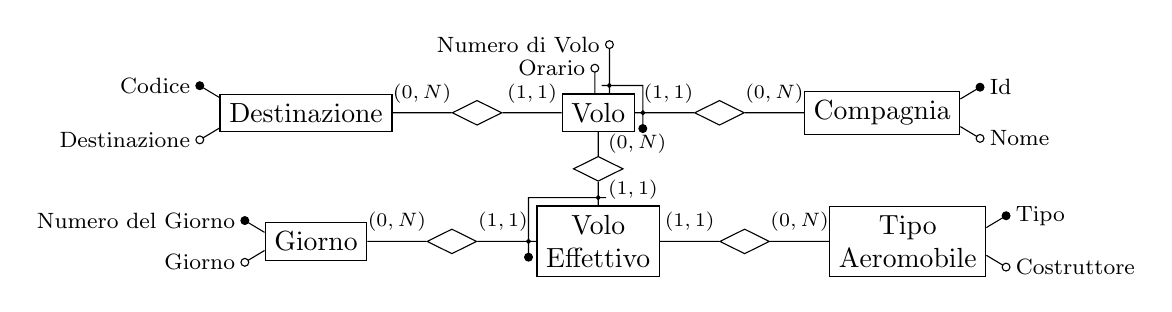
\begin{tikzpicture}
    \draw

    %%* Attributi:
    %%  node[draw, circle, inner sep=1pt, fill=black]{}node[right]{\footnotesize A}
    %%? Distanza orizzontale: E -(0.25,0.x)- A
    %%? Distanza verticale: E -(0,x * 0.22)- A

    %%* Cardinalità:
    %%  node[below right]{\scriptsize $(0,N)$}
    %%  node[above right]{\scriptsize $(0,N)$}
    %%  node[midway, above]{\scriptsize $(0,N)$}

    %%* Relazione:
    %%  node[draw, diamond, shape aspect=2, inner sep=3pt, anchor=90](r1){}
    %%  node[draw, diamond, shape aspect=2, inner sep=0.2pt, anchor=180](r2){R2}

    %%* Entità:
    %%  node[draw, rectangle, anchor=90](e1){}
    %%? Distanza verticale: E -(0.3)- R -(0.3) E
    %%? Distanza orizzontale: E -(0.75)- R -(0.75)- E

    %%* Destinazione
    (0,0)node[draw, rectangle, anchor=180](e1){Destinazione}
    (e1.0)--++(0.75,0)node[draw, diamond, shape aspect=2, inner sep=3pt, anchor=180](r1){}node[midway, above]{\scriptsize $(0,N)$}

    (e1.190)--++(-0.25,-0.15)node[draw, circle, inner sep=1pt, fill=white]{}node[left]{\footnotesize Destinazione}
    (e1.170)--++(-0.25,0.15) node[draw, circle, inner sep=1pt, fill=black]{}node[left]{\footnotesize Codice}

    %%* Volo
    (r1.0)--++(0.75,0)node[draw, rectangle, anchor=180](e2){Volo}node[midway, above]{\scriptsize $(1,1)$}
    (e2.0)--++(0.1,0)node[draw, circle, inner sep=0.5pt, fill=black](a){}--++(0.65,0)node[draw, diamond, shape aspect=2, inner sep=3pt, anchor=180](r2){}node[midway, above]{\scriptsize $(1,1)$}

    (e2.100)--++(0,0.32)node[draw, circle, inner sep=1pt, fill=white]{}node[left]{\footnotesize Orario}
    (e2.60)--++(0,0.1)node[draw, circle, inner sep=0.5pt, fill=black](b){}--++(0,0.52)node[draw, circle, inner sep=1pt, fill=white]{}node[left]{\footnotesize Numero di Volo}

    (a)++(0,-0.2)node[draw, circle, inner sep=1pt, fill=black]{}|-(b)--++(-0.1,0)

    %%* Compagnia
    (r2.0)--++(0.75,0)node[draw, rectangle, anchor=180](e3){Compagnia}node[midway, above]{\scriptsize $(0,N)$}

    (e3.350)--++(0.25,-0.15)node[draw, circle, inner sep=1pt, fill=white]{}node[right]{\footnotesize Nome}
    (e3.10)--++(0.25,0.15) node[draw, circle, inner sep=1pt, fill=black]{}node[right]{\footnotesize Id}

    %%* Volo Effettivo
    (e2.270)--++(0,-0.3)node[draw, diamond, shape aspect=2, inner sep=3pt, anchor=90](r3){}node[midway, right]{\scriptsize $(0,N)$}
    (r3.270)--++(0,-0.2)node[draw, circle, inner sep=0.5pt, fill=black](a){}node[midway, right]{\scriptsize $(1,1)$}--++(0,-0.1)node[draw, rectangle, anchor=90, align=center](e4){Volo\\Effettivo}


    %%* Giorno
    (e4.180)--++(-0.1,0)node[draw, circle, inner sep=0.5pt, fill=black](b){}--++(-0.65,0)node[draw, diamond, shape aspect=2, inner sep=3pt, anchor=0](r4){}node[midway, above]{\scriptsize $(1,1)$}
    (r4.180)--++(-0.75,0)node[draw, rectangle, anchor=0](e5){Giorno}node[midway, above]{\scriptsize $(0,N)$}
    
    (e5.190)--++(-0.25,-0.15)node[draw, circle, inner sep=1pt, fill=white]{}node[left]{\footnotesize Giorno}
    (e5.170)--++(-0.25,0.15) node[draw, circle, inner sep=1pt, fill=black]{}node[left]{\footnotesize Numero del Giorno}

    (b)++(0,-0.2)node[draw, circle, inner sep=1pt, fill=black]{}|-(a)--++(0.1,0)

    %%* Tipo Aeromobile
    (e4.0)--++(0.75,0)node[draw, diamond, shape aspect=2, inner sep=3pt, anchor=180](r5){}node[midway, above]{\scriptsize $(1,1)$}
    (r5.0)--++(0.75,0)node[draw, rectangle, anchor=180,align=center](e6){Tipo\\Aeromobile}node[midway, above]{\scriptsize $(0,N)$}

    (e6.350)--++(0.25,-0.15)node[draw, circle, inner sep=1pt, fill=white]{}node[right]{\footnotesize Costruttore}
    (e6.10)--++(0.25,0.15) node[draw, circle, inner sep=1pt, fill=black]{}node[right]{\footnotesize Tipo}

    ;
\end{tikzpicture}
\end{document}